
\documentclass[a4paper,12pt]{article}
\usepackage[utf8]{inputenc}
\usepackage[ngerman]{babel}
\usepackage{hyperref}
\usepackage{xcolor} 
\usepackage{graphicx}
\usepackage{geometry}

\geometry{a4paper, margin=0.5in}

\title{Technische Spezifikationen und Analyse der Intel RealSense Depth Camera D435}
\author{}
\date{}

\begin{document}

\maketitle
% \section*{Intel RealSense Depth Camera D435}


\begin{center}

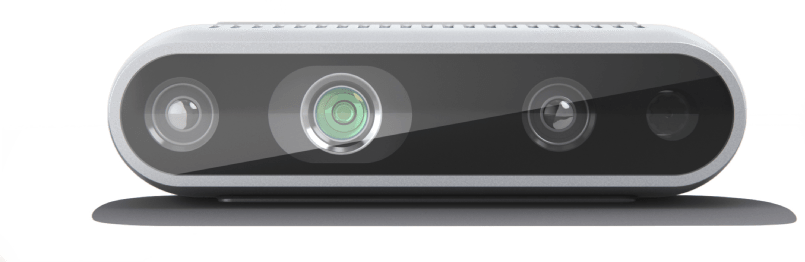
\includegraphics[width=0.8\textwidth]{./Bilder/d435-3.png}

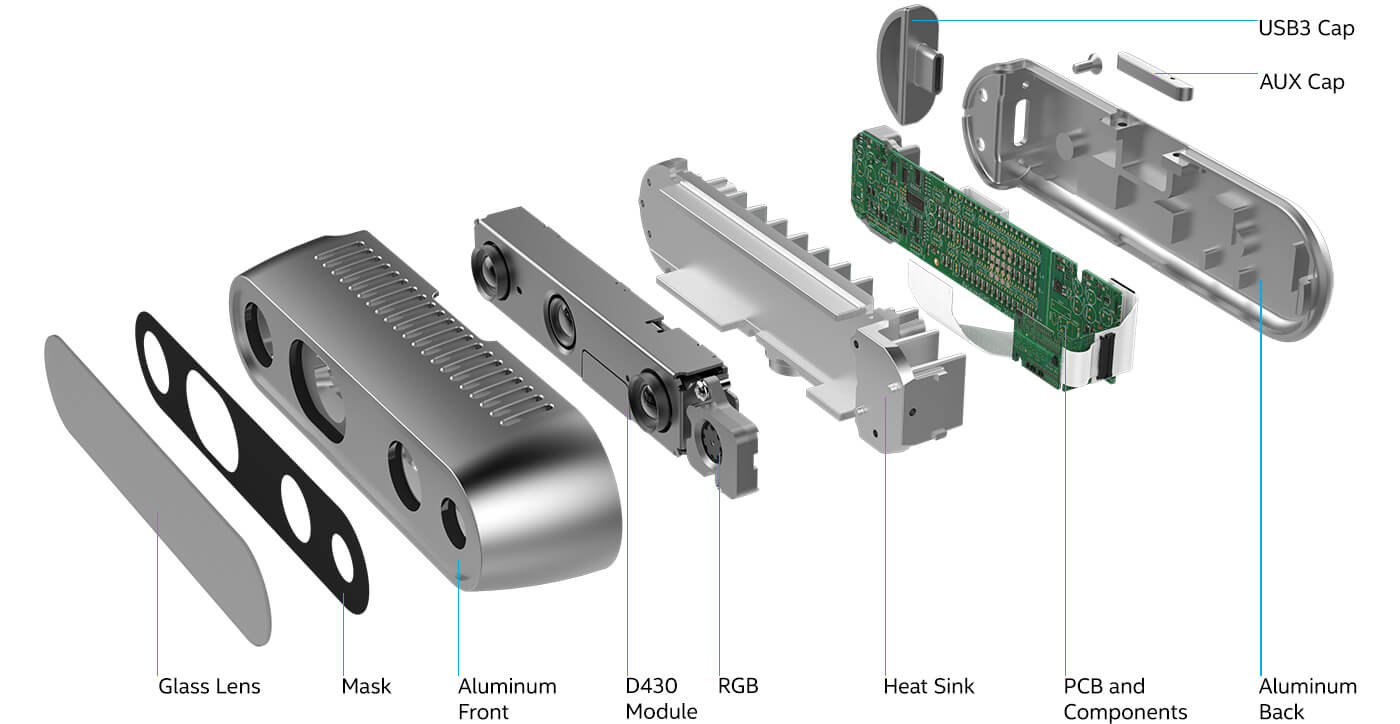
\includegraphics[width=0.8\textwidth]{./Bilder/d435_2.jpg}

\end{center}

\section*{Technische Daten}

\begin{itemize}
    \item \textbf{Tiefensensor:}
    \begin{itemize}
        \item \textbf{Technologie:} Aktive Stereoskopie
        \item \textbf{Auflösung:} Bis zu 1280 × 720 Pixel
        \item \textbf{Bildrate:} Bis zu 90 Bilder pro Sekunde
        \item \textbf{Sichtfeld (FOV):} Horizontal 85,2°, Vertikal 58°
        \item \textbf{Empfohlener Arbeitsbereich:} 0,3 m bis 3 m
    \end{itemize}
    \item \textbf{RGB-Sensor:}
    \begin{itemize}
        \item \textbf{Auflösung:} 1920 × 1080 Pixel
        \item \textbf{Bildrate:} 30 Bilder pro Sekunde
        \item \textbf{Technologie:} Rolling Shutter
        \item \textbf{Sichtfeld (FOV):} Horizontal 69°, Vertikal 42°
    \end{itemize}
    \item \textbf{Physische Eigenschaften:}
    \begin{itemize}
        \item \textbf{Abmessungen:} 42 mm × 42 mm × 23 mm
        \item \textbf{Gewicht:} 60 g
        \item \textbf{Anschluss:} USB 3.0
    \end{itemize}
    \item \textbf{Besondere Merkmale:}
    \begin{itemize}
        \item \textbf{Global Shutter:} Für Tiefensensoren, ermöglicht genaue Tiefenerfassung bei bewegten 
        Objekten oder Kamerabewegungen
        \item \textbf{Weites Sichtfeld:} Ermöglicht die Erfassung größerer Szenen und minimiert „tote Winkel“
        \item \textbf{Einsatzbereich:} Geeignet für Innen- und Außenanwendungen
    \end{itemize}
\end{itemize}

\section*{Gründe für die Wahl der Intel RealSense Depth Camera D435}

\begin{enumerate}
    \item \textbf{Präzise Tiefenerfassung:} Dank der aktiven Stereoskopie und des Global Shutters kann 
    die D435 genaue Tiefendaten liefern, selbst bei schnellen Bewegungen oder in dynamischen Umgebungen.
    \item \textbf{Weites Sichtfeld:} Das horizontale Sichtfeld von 85,2° ermöglicht es Robotern, ein 
    größeres Umfeld zu erfassen, was für die Navigation und Objekterkennung in industriellen 
    Anwendungen vorteilhaft ist.
    \item \textbf{Hohe Bildrate:} Mit bis zu 90 Bildern pro Sekunde in der Tiefenerfassung kann die 
    Kamera schnelle Prozesse in Echtzeit überwachen, was in industriellen Anwendungen entscheidend sein kann.
    \item \textbf{Kompakte Bauweise:} Die geringen Abmessungen und das leichte Gewicht erleichtern 
    die Integration der Kamera in verschiedene Robotersysteme, ohne das Design wesentlich zu beeinflussen.
    \item \textbf{Vielseitigkeit:} Die Fähigkeit, sowohl in Innen- als auch in Außenumgebungen zu arbeiten, 
    erweitert die Einsatzmöglichkeiten der Kamera in unterschiedlichen industriellen Szenarien.
    \item \textbf{Einfache Integration:} Der USB 3.0-Anschluss und die Kompatibilität mit verschiedenen 
    Softwareplattformen ermöglichen eine nahtlose Integration in bestehende Systeme.
\end{enumerate}

\section*{Quellen}
\textcolor{blue}{\href{https://www.intelrealsense.com/depth-camera-d435/}{Intel® RealSense™ Depth Camera D435}}
\end{document}
